%! LuaLaTeX 文書
\documentclass[unicode,colorlinks]{beamer}
\usetheme{metropolis}
\usefonttheme{professionalfonts}

\hypersetup{linkcolor=blue,urlcolor=teal}

\usepackage{luatexja}
\ltjsetparameter{jacharrange={-2,-3,-8}}
\usepackage[no-math,match,deluxe]{luatexja-preset}

\usepackage{graphicx,xcolor}
\usepackage{pxrubrica}
\usepackage{tcolorbox}
\usepackage{bxwareki}

\usepackage{tikz}
\usetikzlibrary{plotmarks}

\usepackage{bxokumacro}
\usepackage{keystroke}

\usepackage[T1]{fontenc}
\usepackage{amsmath,mathtools,amssymb,mathrsfs,rsfso,mleftright}
\usepackage[math]{kurier}
\usepackage[euler-digits]{eulervm}
\usepackage[scaled]{beramono}
\allowdisplaybreaks[4]

%%%%%%%%%% 商用フォントを用いているので、自分でタイプセットする場合は適当に以下を変えてください
\setmainfont[
	Ligatures=TeX,
	BoldFont=FOT-RodinNTLGPro-EB,
	ItalicFont=FOT-RodinNTLGPro-EB,
]{FOT-RodinNTLGPro-B}
\setsansfont[
	Ligatures=TeX,
	BoldFont=FOT-RodinNTLGPro-EB,
	ItalicFont=FOT-RodinNTLGPro-EB,
]{FOT-RodinNTLGPro-B}
\setmainjfont[
	Ligatures=TeX,
	CharacterWidth=Proportional,
	JFM=prop,
	BoldFont=FOT-RodinNTLGPro-EB,
	ItalicFont=FOT-RodinNTLGPro-EB,
]{FOT-RodinNTLGPro-B}
\setsansjfont[
	Ligatures=TeX,
	CharacterWidth=Proportional,
	JFM=prop,
	BoldFont=FOT-RodinNTLGPro-EB,
	ItalicFont=FOT-RodinNTLGPro-EB,
]{FOT-RodinNTLGPro-B}
\setmonofont[
	Ligatures=TeX
]{DejaVu Sans Mono}
\setmonojfont[
	Ligatures=TeX,
]{NotoSansMonoCJKjp-Regular}

%%%%%%%%%% 以下は自前コマンド

\newcommand{\centeralign}[1]{\rule{0pt}{0pt}\hfill#1\hfill\rule{0pt}{0pt}}
\newcommand{\Unit}[1]{\,\mathrm{#1}}

\setlength{\parskip}{2ex}

\title{大気放射の基礎\\--Liou著 藤枝・深堀訳 (2014) の講読--}
\author{北海道大学理学部 人見祥磨}
\date{\warekitoday}

\begin{document}
\maketitle

\begin{frame}{目次}
	\tableofcontents
\end{frame}

\section{線の広がり}

\begin{frame}
	\frametitle{線の広がり}
	単色の射出は現実には観測されない。

	原子や分子への外部からの影響と、射出の際のエネルギー損失のため、
	エネルギー遷移する間にエネルギー準位が僅かに変化する。

	その結果、非単色の放射となり、有限の幅を持つスペクトル線が観測される。
\end{frame}

\begin{frame}
	\frametitle{ローレンツ線形}
	ローレンツ線形: 圧力による広がり。衝突によって広げられたスペクトル線の線形。

	\[k_\nu=\frac{S}{\pi}\frac{\alpha}{(\nu-\nu_0)^2+\alpha^2}=Sf[\nu-\nu_0]\]

	$k_\nu$: 吸収係数 ;\quad $\nu_0$: 理想的な単色の吸収線の波数;\\
	$\alpha$: 吸収線の半値半幅:(圧力と温度の関数);\\
	$f$: 形状因子 (shape factor);\quad $\displaystyle S=\int^\infty_{-\infty}k_\nu\,d\nu$: 線強度
\end{frame}

\begin{frame}
	\frametitle{ローレンツ線形}
	\centeralign{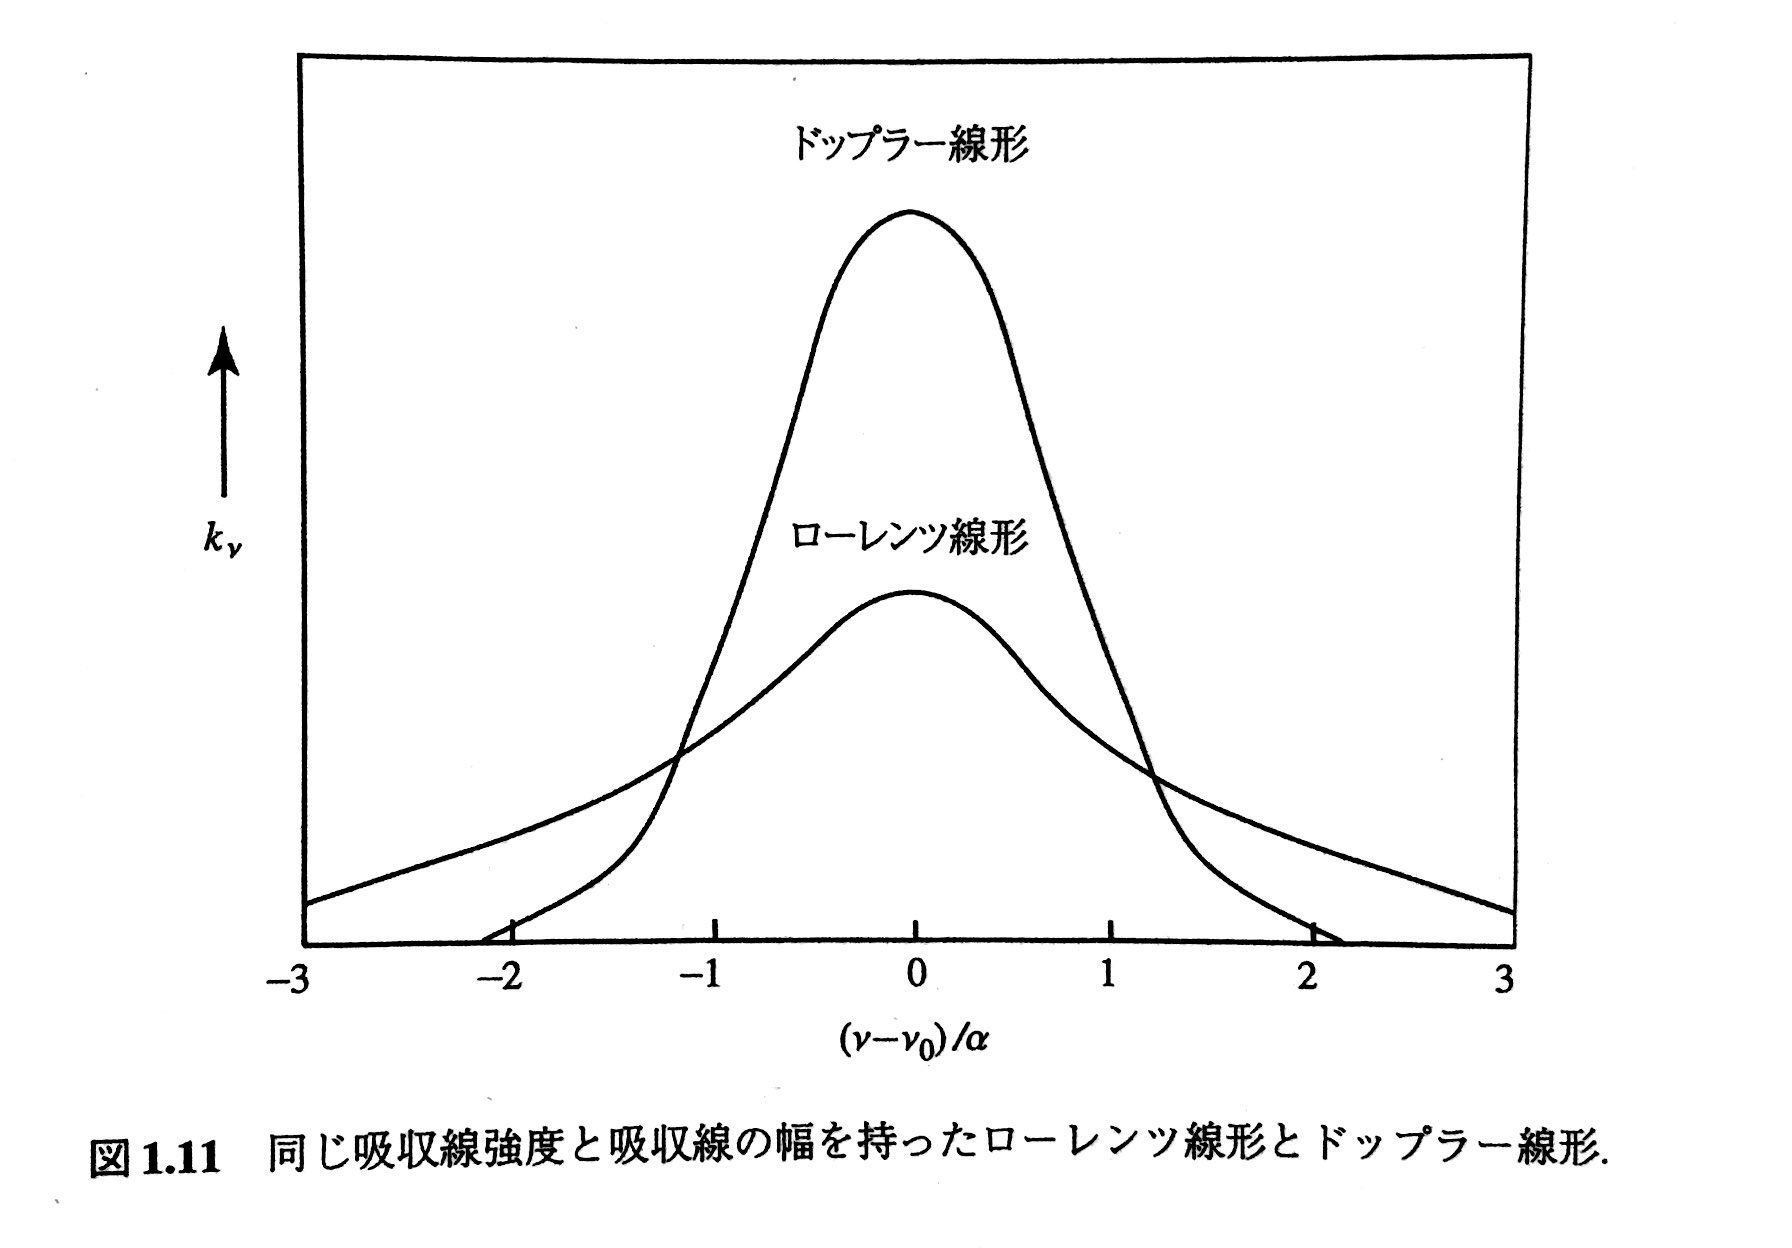
\includegraphics[width=0.8\textwidth]{lorentz.jpg}}
\end{frame}

\section{大気の熱赤外放射伝達}

\begin{frame}
	\frametitle{大気の熱赤外放射伝達}
	アルベド: $\bar r$;\quad 地球半径: $a_e$;\quad\\
	太陽定数: $S=1366\Unit{W\,m^{-2}}$;\quad 地球大気系の平衡温度: $T_e$
	\begin{block}{放射に関してのバランス方程式}
		ステファン・ボルツマンの法則から
		\[S\cdot\pi{a_e}^2(1-\bar r)=\sigma{T_e}^4\cdot4\pi{a_e}^2\]
		係数$4$: 吸収と射出の面積の違い

		バランス方程式より、
		\[T_e=\sqrt[4]{S\frac{1-\bar r}{4\sigma}}\sim255\Unit{K}\]
	\end{block}
\end{frame}

\begin{frame}
	\frametitle{放射伝達のための一般的な方程式}
	放射束の放射強度: $I_\nu$;\quad 吸収係数: $k_\nu$;\\
	吸収気体の密度: $\rho_a$;\quad 光路長: $s$;\quad 放射源関数: $J_\nu$
	\[-\frac{1}{k_\nu \rho_a}\frac{dI_\nu}{ds}=I_\nu-J_\nu\]

	\begin{description}
		\item[放射強度] 時間に依存しないと考えて良い
		\item[平行平面大気] 放射強度と大気パラメーターは鉛直方向にのみ変化
	\end{description}
\end{frame}

\end{document}
